\documentclass[12pt]{article}
\usepackage[top=1in, bottom=1in, left=1in, right=1in]{geometry}

\usepackage{setspace}
\onehalfspacing

\usepackage{amssymb}
%% The amsthm package provides extended theorem environments
\usepackage{amsthm}
\usepackage{epsfig}
\usepackage{times}
\renewcommand{\ttdefault}{cmtt}
\usepackage{amsmath}
\usepackage{graphicx} % for graphics files

% Draw figures yourself
\usepackage{tikz} 

% writing elements
\usepackage{mhchem}

\usepackage{paralist}

% The float package HAS to load before hyperref
\usepackage{float} % for psuedocode formatting
\usepackage{xspace}

% from Denovo Methods Manual
\usepackage{mathrsfs}
\usepackage[mathcal]{euscript}
\usepackage{color}
\usepackage{array}

\usepackage[pdftex]{hyperref}
\usepackage[parfill]{parskip}

% math syntax
\newcommand{\nth}{n\ensuremath{^{\text{th}}} }
\newcommand{\ve}[1]{\ensuremath{\mathbf{#1}}}
\newcommand{\Macro}{\ensuremath{\Sigma}}
\newcommand{\rvec}{\ensuremath{\vec{r}}}
\newcommand{\omvec}{\ensuremath{\hat{\Omega}}}
\newcommand{\vOmega}{\ensuremath{\hat{\Omega}}}
%---------------------------------------------------------------------------
%---------------------------------------------------------------------------
\begin{document}
\begin{center}
{\bf NE 255, Fa16 \\
Simplifying the Transport Equation\\
September 15, 2016}
\end{center}

\setlength{\unitlength}{1in}
\begin{picture}(6,.1) 
\put(0,0) {\line(1,0){6.25}}         
\end{picture}

Recall that last time we created a full version of the transport equation that looked like: 
\begin{align}
&\frac{1}{v}\frac{\partial \psi}{\partial t}(\rvec,E,\omvec,t) + \omvec\cdot  \nabla \psi(\rvec,E,\omvec,t) +
 \Sigma_t(\rvec,E)\psi(\rvec,E,\omvec,t) 
\\& \quad\quad\quad\quad =
\int_0^{\infty}\int_{4\pi}\Sigma_s(\rvec, E'\rightarrow E,\omvec'\rightarrow\omvec)
\psi(\rvec,E',\omvec',t)d\omvec'dE'\nonumber
\\&\quad\quad\quad\quad\quad\quad +\frac{\chi_p(E)}{4\pi}\int_0^{\infty}\int_{4\pi}\nu(E')\Sigma_f(\rvec,E')
\psi(\rvec,E',\omvec',t)d\omvec'dE'\nonumber
\\&\quad\quad\quad\quad\quad\quad\quad\quad+S(\rvec, E, \omvec,t) \nonumber.
\end{align}
What does each term describe?

We talked a little bit about boundary and initial conditions, and I was teaching from a non-updated version of the notes. Here's what I missed: (see notes posted online, which are now up-to-date)...

%----------------------------------------------
\section*{Simplified Forms}
At the end of class we went briefly into simplifications; we're going to spend more time on that in this class. 

\subsection*{Time Independent}
We'll spend most of our time on this version of the equation. We assume that losses and sources are balanced, and thus there is no rate of change with time:
\[\frac{\partial \psi}{\partial t} = 0\]
We can then remove the time dependence from all terms in our equation. As noted, for reactors we often 
\begin{compactitem}
\item solve a steady-state form of the equation,
\item perform depletion calculations that characterize material evolution (using the Batemann equations, which we're skipping for now)
\item solve a new steady-state calculation with updated material specifications.
\end{compactitem}

\subsection*{One Speed}
Assume all particles are at the same speed, $\vec{v} = v_0 \cdot \vOmega$. Thus
\begin{align*}
n(\vec{r}, v, \vOmega, t) &= n(\vec{r}, \vOmega, t) \delta(v - v_0) \\
\Sigma_s(E' \rightarrow E, \vOmega' \rightarrow \vOmega) &= \Sigma_s(E, \vOmega' \rightarrow \vOmega)\delta(E' - E)
\end{align*}
%
Now we can remove E integration and E dependence:
%
\begin{align*}
\frac{1}{v}\frac{\partial \psi(\vec{r}, \vOmega, t)}{\partial t} &+ 
\vOmega \cdot \nabla \psi(\vec{r}, \vOmega, t) +
\Sigma_t \psi(\vec{r}, \vOmega, t) = \nonumber\\
%
& \int_{4\pi} d\vOmega' \Sigma_s(\vOmega' \rightarrow \vOmega) \psi(\vec{r}, \vOmega', t)  
+ \frac{\nu \Sigma_f}{4\pi} \int_{4\pi} d\vOmega' \psi(\vec{r},  \vOmega', t) 
+ S(\vec{r}, \vOmega, t) 
%Q(\vec{r}, \vOmega, t)
\end{align*}
%
%Where:
%\begin{align}
%Q(\vec{r}, \vOmega, t) &= \frac{1}{4\pi} \nu \Sigma_f \int_{4\pi} d\vOmega' \psi(\vec{r},  \vOmega, t) + S(\vec{r}, \vOmega, t) \\
%&= \frac{1}{4\pi} \bigl( \nu \Sigma_f \phi(\vec{r}, t) + s(\vec{r}, t) \bigr)
%\end{align}

\subsection*{Isotropic Source}
It is often the case that an external source is (or we can approximate it as) isotropic:
\[ S(\vec{r}, E, \vOmega, t) = \frac{1}{4 \pi}  S(\vec{r}, E, t) \]


%---------------------------------------------
\subsection*{One Dimensional and Rotational (Azimuthal) Symmetry}
We also often simplify by only worrying about fewer dimensions. Here we'll look at just one: we'll get rid of $x$ and $y$. Let's remind ourselves of how phase-space looks (see \autoref{fig:phase_space}):
\begin{figure}[h!]
    \begin{center}
    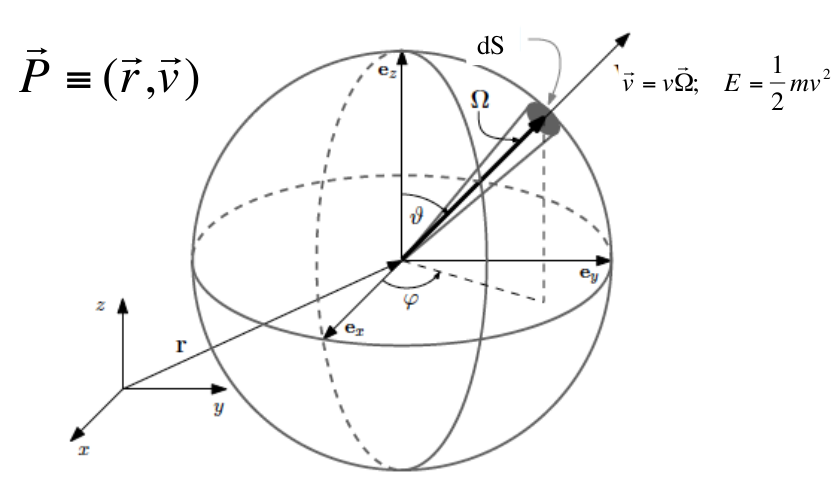
\includegraphics[keepaspectratio, width = 4 in]{phase-space}
    \end{center}
    \caption{Schematic of Phase Space}
    \label{fig:phase_space}
\end{figure}

We first assume that \textbf{things only vary in the $z$ dimension}, so $\vec{r} \rightarrow z$, e.g.\\ $\psi(\vec{r}, E, \vOmega, t) \rightarrow \psi(z, E, \vOmega, t)$

We next assume (which is often true) that our systems is \textbf{azimuthally symmetric} (see \autoref{fig:azimuthal}), which means that the scattering only depends on the angle of the scattering cosine, $\mu =\vOmega' \cdot \vOmega$, because it is symmetric about the azimuthal direction ($\varphi$). We can use this assumption to simplify two things. 
\begin{figure}[h!]
    \begin{center}
    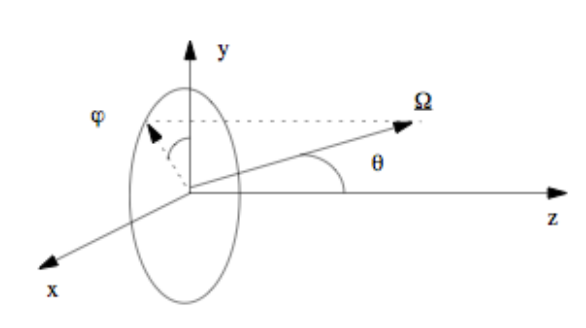
\includegraphics[keepaspectratio, width = 3 in]{azimuthal}
    \end{center}
    \caption{Azimuthal symmetry}
    \label{fig:azimuthal}
\end{figure}

We will use these terms in our simplifications:\\
$d\vOmega = \sin(\theta) d\theta d\varphi = d\mu d\varphi; \quad \mu = \cos(\theta)\,$ so $d\mu = \sin(\theta)\:; \quad \Omega_x = \cos(\theta) = \mu\:.$
\begin{align*}
\int_{4 \pi} d\vOmega &= \int_0^{2\pi} d\varphi \int_{-\pi/2}^{\pi/2} \sin(\theta) d\theta =  \int_0^{2\pi} d\varphi \int_{-1}^1 d\mu = 4\pi \\
\psi(z,\vOmega,E,t) d\vOmega &= \psi(z,\varphi, \mu,E,t) d\varphi  d\mu =  \psi(z, \mu,E,t) d\varphi  d\mu 
\end{align*}
%
With azimuthal symmetry we can rewrite the scattering cross section since it is no longer a function of $\varphi$.
\[\Sigma_s(z, \vOmega' \rightarrow \vOmega) \rightarrow \Sigma_s(z, \vOmega' \cdot \vOmega) = \Sigma_s(z, \mu) \:.\]

Further, we can execute the angular integration over $\varphi$ since nothing depends on it anymore. For example:
\begin{align*}
\int_{4 \pi} d\vOmega\: \psi(z, \vOmega, E, t) &=   \int_0^{2\pi} d\varphi \int_{-1}^1 d\mu \:\psi(z, \vOmega, E, t) \\
&= 2 \pi \int_{-1}^1 d\mu \:\psi(z, \vOmega, E, t)\\
\psi(z, \mu, E, t) &= \frac{1}{2 \pi}\psi(z, \vOmega, E, t)\:.
\end{align*}
%
The next simplification is in the streaming term:
\[\vOmega \cdot \nabla \psi(\vec{r}, \vOmega, E, t) \rightarrow \Omega_z \frac{\partial \psi(z, \vOmega, E, t)}{\partial z} = \mu \frac{\partial \psi(z, \vOmega, E, t)}{\partial z} \]
%
We can combine all of this into a 1-D equation, using $\mu_0 = \vOmega \cdot \vOmega'$:
\begin{align*}
\frac{1}{v}\frac{\partial \psi}{\partial t}(z,E,\omvec,t) &+ \Omega_z \frac{\partial \psi(z, \vOmega, E, t)}{\partial z} + \Sigma_t(z)\psi(z, \vOmega, E, t)  \\
&= \frac{\chi(E)}{4 \pi} \int_0^{\infty} dE'\int_{4 \pi} d\vOmega'\:  \nu(E')\Sigma_f(z,E',t)\psi(z, \vOmega', E', t)  \\
&+ \int_0^{\infty} dE' \int_{4 \pi} d\vOmega'\: \Sigma_s(z, \mu_0)\psi(z, \vOmega', E', t) + S(z, E, \vOmega, t)\:,
\end{align*}
%
which we can then integrate over the $\varphi$ component of angle:
\begin{align*}
\frac{1}{v}\frac{\partial \psi}{\partial t}(z,E,\omvec,t) &+ \mu \frac{\partial \psi(z, \mu, E, t)}{\partial z} + \Sigma_t(z)\psi(z, \mu, E, t) \\
&= 2\pi\frac{\chi(E)}{4 \pi} \int_0^{\infty} dE' \: \nu(E')\Sigma_f(z,E',t) \int_{-1}^1 d\mu'\: \psi(z, \mu', E', t) \\
&+ 2\pi\int_0^{\infty} dE' \int_{-1}^1 d\mu'\: \Sigma_s(z, \mu_0)\psi(z, \mu', E', t)  + 2\pi S(z, E, \mu, t)
\end{align*}
%
The fission terms becomes
\[\frac{\chi(E)}{2} \int_0^{\infty} dE'\:  \nu(E')\Sigma_f(z,E',t)\underbrace{\phi(z, E', t)}_{\text{scalar flux}}\:. \]
And, if we have an isotropic source
\[2\pi S(z, E, \mu, t) \rightarrow \frac{S(z, E, t)}{2}\:. \]

\subsection*{Combination}
If we combine one-speed, time-independent, isotropic source, one-dimensional, and azimuthally symmetric, we get
\begin{align*}
\mu \frac{\partial \psi(z, \mu)}{\partial z} &+ \Sigma_t(z)\psi(z, \mu) = \\
&\frac{\nu\Sigma_f(z) }{2}\phi(z) + 2\pi\int_{-1}^1 d\mu'\: \Sigma_s(z, \mu_0)\psi(z, \mu')  + \frac{S(z)}{2} \:.
\end{align*}

% \vec{r} switched to x
%\begin{align*}
%\frac{1}{v}\frac{\partial \psi(x, \vOmega, t)}{\partial t} &+ 
%\bigl(\Omega_x \frac{\partial}{\partial x} + \cancel{\Omega_y \frac{\partial}{\partial y}} + \cancel{\Omega_z \frac{\partial}{\partial z}} \bigr)\psi(x, \vOmega, t) +
%\Sigma_t \psi(x, \vOmega, t) = \nonumber\\
%%
%& \int_{4\pi} d\vOmega' \Sigma_s(\vOmega' \rightarrow \vOmega) \psi(x, \vOmega', t)  + 
%\frac{\nu \Sigma_f}{4\pi} \int_{4\pi} d\vOmega' \psi(x,  \vOmega', t) + s(x, \vOmega, t)%+ Q(x, \vOmega, t) \nonumber
%\end{align*}


%\begin{minipage}{0.3\textwidth}
%\begin{figure}[H]
%\includegraphics[height=1.5in]{AzimuthalSymmetry}
%%\caption{\label{fig:FixedCondition} Fixed Condition}
%\end{figure}
%\end{minipage} \hfill
%\begin{minipage}{0.65\textwidth}
%
%\end{minipage}
%
%Using this idea we can write things more cleanly:
%%
%% switch to just \mu
%\begin{align*}
%\frac{1}{v_0}\frac{\partial \psi(x, \vOmega, t)}{\partial t} &+ 
%\mu \frac{\partial}{\partial x}\psi(x, \vOmega, t) +
%\Sigma_t \psi(x, \vOmega, t) = \nonumber\\
%%
%& \int_0^{2\pi} d\phi \int_{4\pi} d\vOmega' \Sigma_s(\vOmega' \cdot \vOmega) \frac{\psi(x, \mu', t)}{2\pi}  + 
%\frac{1}{4\pi} \nu \Sigma_f \int_0^{2\pi} d\phi \psi(x, \mu, t) + s(x, \mu, t)% 2\pi Q(x, \mu, t)
%\end{align*}
%
%If \textbf{scattering is also isotropic}:
%\[\Sigma_s(\vOmega' \cdot \vOmega) = \frac{\Sigma_s}{4\pi} \]
%
%And we get the 1-group, 1-D, isotropic neutron TE:
%%
%% scattering is now iso, add in sources
%\begin{align*}
%\frac{1}{v_0}\frac{\partial \psi(x, \mu, t)}{\partial t} &+ 
%\mu \frac{\partial}{\partial x}\psi(x, \mu, t) +
%\Sigma_t \psi(x, \mu, t) = \nonumber\\
%%
%& \frac{1}{2} \Sigma_s \int_{-1}^{1} d\mu' \psi(x, \mu', t)  
%+  \frac{1}{2} \bigl( \nu \Sigma_f \phi(x, t) + S(x, t) \bigr)
%\end{align*}
%
%%---------------------------------------------
%\subsection*{Steady State}
%If we get rid of time dependence.
%%
%\begin{equation}
%\mu \frac{\partial}{\partial x}\psi(x, \mu) +
%\Sigma_t \psi(x, \mu) = \frac{1}{2} \Sigma_s \int_{-1}^{1} d\mu' \psi(x, \mu')  
%+  \frac{1}{2} \bigl( \nu \Sigma_f \phi(x) + S(x) \bigr) \nonumber
%\end{equation}
%
%
%And very finally - we can have the unrealistic case of \textbf{purely absorbing media}:
%%
%\begin{equation}
%\mu \frac{\partial}{\partial x}\psi(x, \mu) +
%\Sigma_a \psi(x, \mu) = \frac{1}{2} \bigl( \nu \Sigma_f \phi(x) + S(x) \bigr) \nonumber
%\end{equation}


\end{document}
